\subsubsection{Typ- und Methoden-Konvertierungsvarianten}
Die Konvertierung der einzelnen Type-Matcher liefert eine Menge von so genannten Typ-Konvertierungsvarianten. Eine Typ-Konvertierungsvariante beschreibt eine M�glichkeit, wie ein Typ in einen anderen konvertiert werden kann. Zu diesem Zweck enth�lt eine Typ-Konvertierungsvariante zwei Arten von Information: 
\begin{enumerate}
\item Objekterzeugungsrelevante Informationen
\item Methodendelegationsrelevante Informationen
\end{enumerate}
Typ-Konvertierungsvarianten werden von einem konkreten Typ-Matcher f�r jede m�gliche Form der �bereinstimmung erzeugt. Im speziellen Fall des ExactTypeMatchers und des SpecGenTypeMatcher kann, wenn �berhaupt, nur eine Typ-Konvertierungsvariante erzeugt werden. Da die anderen Typ-Matcher intern wiederum eine �bereinstimmung von Typen fordern, sind von diesen mehrere Typ-Konvertierungsvarianten zu erwarten.\\\\
Die objekterzeugungsrelevanten Informationen sorgen daf�r, dass das Proxy-Objekt zum Source-Typ korrekt erzeugt werden kann.\\\\
Die methodendelegationsrelevanten Informationen werden verwendet um so genannten Methoden-Konvertierungsvarianten zu erzeugen. Diese sorgen daf�r, dass das R�ckgabe-Objekt und die Parameter-Objekte beim Methodenaufruf korrekt konvertiert werden und dass der Aufruf an die richtige Methode des Target-Typs delegiert wird.\\\\
In \abbref{konvar_voll} ist dieser Zusammenhang f�r ein angebotenes Interface AIv und einem erwarteten Interface EI, welche jeweils zwei Methoden enthalten (AM * bzw. EM *), skizziert. Hier wird angenommen, dass jede der angebotenen Methoden strukturell mit jeder der erwarteten Methoden �bereinstimmen w�rde. Dementsprechend enth�lt die Typ-Konvertierungsvariante (TKV) methodendelegationsrelevante Informationen, aus denen insgesamt 4 Methoden-Konvertierungsvarianten erzeugt werden, wovon jede eine Konvertierung entlang der eingezeichneten Pfeile erm�glicht.\\\\
Dabei gilt jedoch, aufgrund der �berlegungen zur Kombination von angebotenen Komponenten (siehe auch \abbref{combinated_components}), dass eine Typ-Konvertierungsvariante nicht zu jeder der erwarteten Methoden solche methodendelegationsrelevanten Informationen enth�lt. \abbref{konvar_unv} zeigt einen solchen Fall mit dem angebotenen Interface AIu.
\begin{figure}[H]
\begin{minipage}[b]{.48\linewidth}
  \centering
  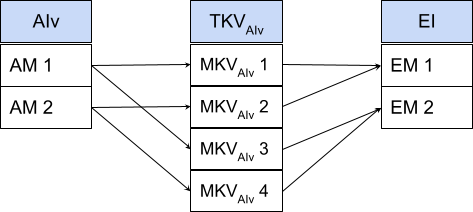
\includegraphics[width=\linewidth]{konvar_voll}
  \caption{Typ- und Methoden-Konvertierungsvarianten von AIv}
  \label{abb:konvar_voll}

\end{minipage}%
\hspace{.04\linewidth}% Abstand zwischen Bilder
\begin{minipage}[b]{.48\linewidth}


  \centering
  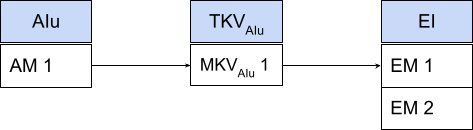
\includegraphics[width=\linewidth]{konvar_unv}
  \caption{Typ- und Methoden-Konvertierungsvarianten von AIu}
  \label{abb:konvar_unv}

\end{minipage}
\end{figure}


